\documentclass[12pt]{article}
\usepackage[margin=1in]{geometry}
\usepackage{amsmath}
\usepackage{amsthm}
\usepackage{float}
\usepackage{graphicx}
\usepackage{multirow}
\usepackage{natbib}
\usepackage{tabularx} 
\usepackage{enumitem}
\usepackage{array}
\usepackage{booktabs}
\usepackage{hyperref}
\usepackage[utf8]{inputenc}
\usepackage{lipsum}
\usepackage[english]{babel}
\usepackage[autostyle, english = american]{csquotes}
\usepackage{underscore}
\MakeOuterQuote{"}
\title{Call Center Regression Data Analysis}

\author{Michael Marcaccio}

\date{November 14 2022}

\begin{document}

\maketitle

\begin{abstract}
 With over 15 million people employed, a predicted compound annual growth rate (CAGR) of 5.6 percent between 2020 and 2027, and with over 28,000 locations
 in the United States alone, call centers play a pivotal role in a business' success.In this paper, call center volume was forecasted and
 models were created to predict the number of agents needed to meet critical attributes such as waittime, calltime, and holdtime. 
 Forecasting gives businesses the ability to make informed business decision and develop data-driven strategies. In the literature it is very
 common to see call center volume being predicted using different techniques, but there is very limited studies on attempting to correlate
 the number of agents needed. Through Regression techniques, there are 8 models proposed to model the number of agents needed based on waittime,
 calltime, goaltime, and the amount of calls handled.
\end{abstract}

\section*{Introduction}
  With over 15 million people employed, a predicted compound annual growth rate (CAGR) of 5.6 percent between 2020 and 2027, and with over 28,000 locations
in the United States alone, call centers play a pivotal role in a business' success. Call centers are a key part of customer service
that will save a company time, money, and unneccessary obstacles. \citep{feinberg2002operational} claims call centers serve as a source of service recovery, added value, market intelligence, and strategic advantage
In the banking industry, calls can range from inquires, transfers, payments, reporting, to processing. This means members could call about their account balance, credit card bills, loan applications, 
or unauthorized transactions. It is crucial that a bank is prepared for spikes in calls and have agents knowledgeable in all aspects of banking and are capable of handling customer impatience. \citep{brown2005statistical} 


  Many studies have been done working with call center volumes as presented in Modeling and Forecasting Call Center Arrivals \citep{ibrahim2016modeling}.
Here an Autoregressive moving average (ARIMA) model is used, which is depicted in the paper as:
\begin{equation}
  \label{eq:ARIMA Standard}
  \Phi(B)(x_i -\mu)=\theta_q(B)\varepsilon_t
\end{equation}
Ibrahim uses multiple ARIMA models to depict seasonality with a combination of exponential smoothing. Holt-Winters smoothing is also used,
with three equations of:
\begin{equation}
  \label{eq:Holt-Winters}
  M_t=\alpha_0(X_t-S_{t-s}) + (1-\alpha_0)(M_{t-1}+B_{t-1}),
\end{equation}
\begin{equation}
  \label{eq:Holt-Winters2}
  B_t=\alpha_1(M_t-M_{t-1}) +(1-\alpha_1)B_{t-1},
\end{equation}
\begin{equation}
  \label{eq:Holt-Winters3}
  S_t=\alpha_2(X_t-M_t) +(1-\alpha_2)S_{t-s},
\end{equation}
where $B_{t}$ is the slope component, $M_{t}$ is the level component, $S_{t}$ is the seasonal component, and s is the period of seasonality.
ARIMA models are a great model to create as "they allow the  representation of a  wide array of potentially useful predictor functions in  models  which contain relatively few parameters" \citep{newbold1983arima}.
With the combination of Holt-Winters smoothing, Ibrahim creates a great model for forecasting call volume, however the paper never goes into detail about
how many agents there should be working at a set time. 

  \citep{evensen1999effective} goes into detail about effective service delivery stating the expectations of customers are a "function of
the customer's own experiences...and when judging their own service quality, financial instiutions need to evalute themselves on 
objective measures which span across industries".When taking this into consideration, I focused my models on using a calls per agent approach,
so agents are not overworked and can treat each caller with respect while answering their concerns in a timely manner to represent the business in a good light. \citep{avramidis2005modeling} confirms
this as it is described as the "call-to-agent assignment problem", and that an efficiency-driven call center is important.


  The contributions of the paper creates models on the basis to maximize quality of service in relation to the number of agents. 
Based on this, models were created to minimize:
\begin{enumerate}
  \item Wait Time
  \item Call Time
  \item Reduce the Amount of Agent Handle Time
  \item Reduce the Amount of Calls not being handled
\end{enumerate}
The remainder of the paper will present the dataset and break it into a clear view on the historical data. I have also created a 
forecast on the projected call volume throughout a week on 15 minute intervals.


\section*{Data}
\begin{sloppypar}
  The data comes from an undisclosed bank where I wrote two SQL queries to obtain. This comes directly from the banks records dating back from Febuary 2020
  to Septemeber 2022, and I was lucky enough to do a data analysis on real-life data. This dataset consists of 466,565 observations of 31 variables. 
  Some significant variables consist of Calldate, Caller_ID, Caller_ID, QueuedYN, AnsweredYN, AbandonedYN, QueuedName, InteractionOutcome, 
  AnsweredGoalMet, StartTime, EndTime, WaitTime, Holdtime, AgentTalkDuration, AgentHandleTime, WrapUpTime, DayoftheYear,
  WeekoftheYear, and NbrofAgents.
\end{sloppypar}
  It is important to acknowledge that AgentTalkDuration refers to the actual amount of time the agent the agent was talking while
AbandonedYN refers to if the caller ended the call before speaking to a representative. The QueuedYN is if the member was put in a queue and had to wait to speak to an agent.
The queue is an automated service or an IVR (Interactive Voice Response). The latest generation of speech-recognition technology allows
IVRs to interpret complex user commands, so customers may be able to “self-serve”, i.e., complete the service interaction at the IVR. \citep{avramidis2005modeling}.
Holdtime is how long the member waits when an agent places on them hold, while waittime is how long they have to wait before someone answers there call.
WrapUpTime refers to how long the member takes to hang up the phone after the agent stops talk. AgentHandleTime is the total of Holdtime, WrapUpTime, and AgentTalkDuration combined.

  This data is allows me to easily answer the research question as I am using real-life data. With a huge sample size and many variables,
this is a great opportunity for data analysis and modeling. With this dataset, I know when doing calculations such as finding means and creating plots, 
I will able to accurately give a truly image of call center volume and agent information to a small period of time such as 15 minutes.
  I did do some exploratory data analysis by creating figures that represent call center volume by the year, month, day of week, and time. 
I also created a table that shows the average wait time, talk time, hold time, wrap up time, and count of every Interaction Outcome.
\begin{figure}[H]
  \centering
  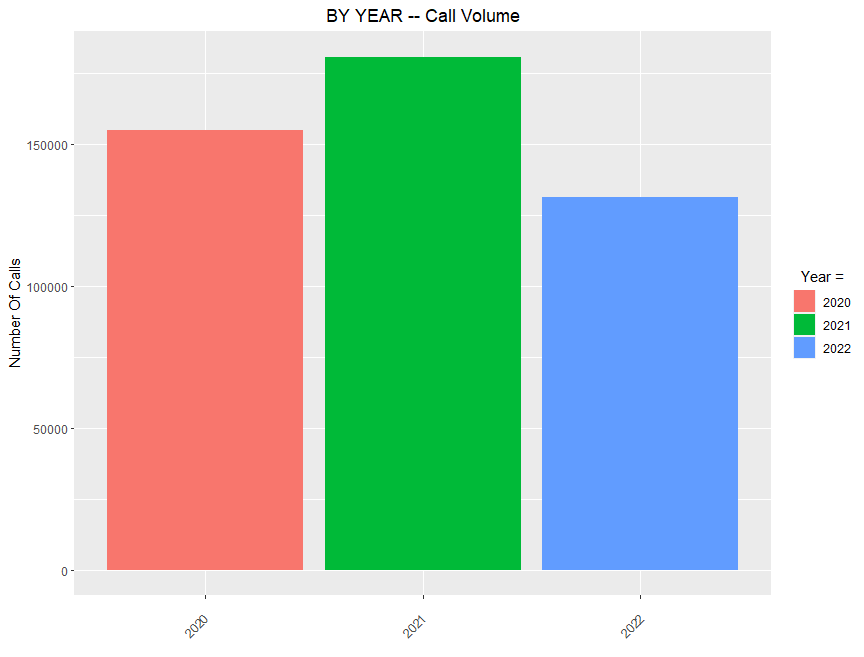
\includegraphics[width=\textwidth]{By Year.png}
  \caption{Call Volume Grouped by Year.}
  \label{fig:Year}
\end{figure}
Here we can see that 2021 has the highest call volume. Please Note that 2020 only has 11 months, while 2020 only has 10. This may be why the data appears skewed.
\begin{figure}[H]
  \centering
  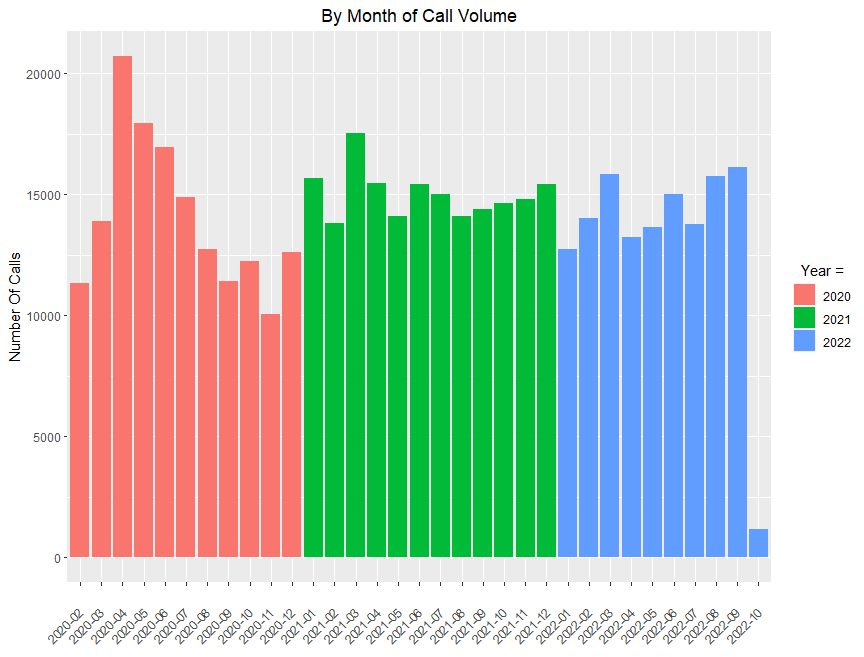
\includegraphics[width=\textwidth]{ByMonthVolume.png}
  \caption{Call Volume Grouped by Month.}
  \label{fig:Month}
\end{figure}
When grouped by month, we can see an interesting peak around April. This may be because that is tax season and members are calling for tax information.
Also April 2020 may have a higher peak than April 2021, due to COVID-19. During that time, many individuals were eligble for a 1,200 dollar stimulus check.
\begin{figure}[H]
  \centering
  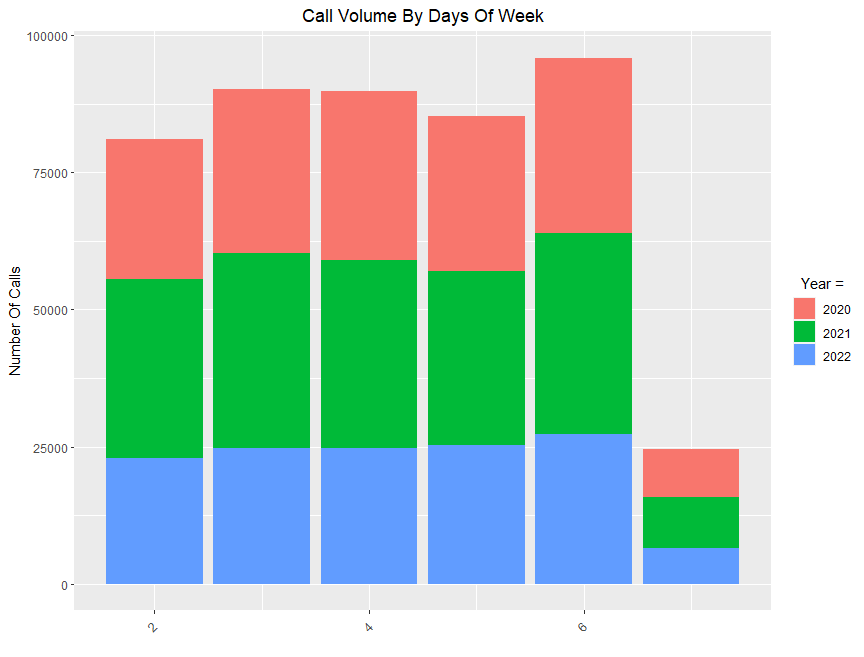
\includegraphics[width=\textwidth]{CallVolumeByDayOfWeek.png}
  \caption{Call Volume Grouped by Day.}
  \label{fig:Day}
\end{figure}
With Sunday representing 1, we can see that most calls happen on a Friday. Saturday has an extremely low count. This can be explained due to the
varying hours of the call center. Monday through Thursday, the call center is open 8am to 5pm, a total of 9 hours. Friday the call center is open
8am-7pm, a total of 11 hours. Saturday the call center is only open 8:30 am to 12pm, a total of 3 and a half hours.
\begin{figure}[H]
  \centering
  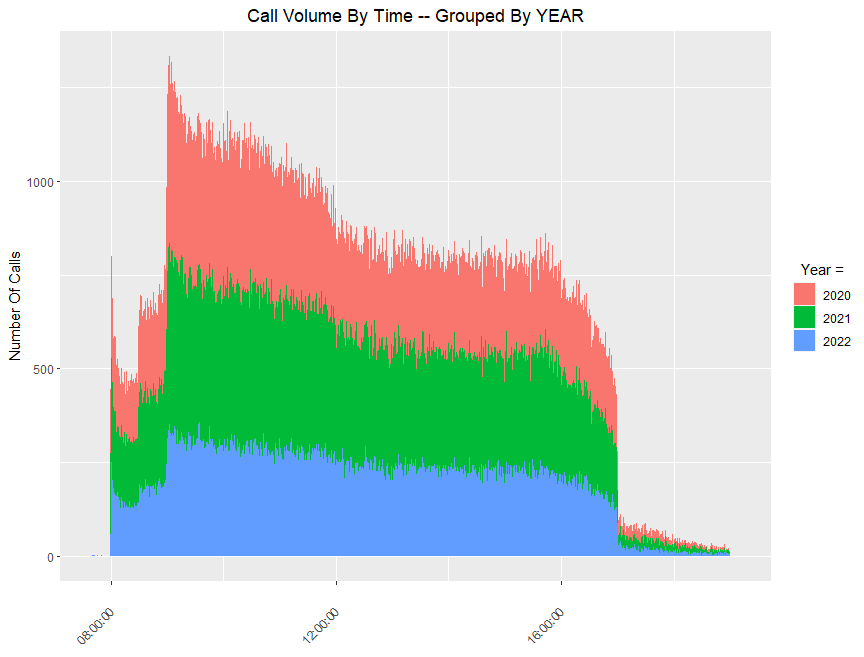
\includegraphics[width=\textwidth]{CallVolumeByTimeOfDayGROUPEDbyYear.png}
  \caption{Call Volume Grouped by Time.}
  \label{fig:Timeoneday}
\end{figure}
The call center consistently has a spike around 9am throughout the 3 years. This is suprising as the call center opens at 8am. This is important to be aware of when
creating a forecasting model and having the banks employees be at their station at 9am. The decreasing trend throughout the day is not suprising
as most people are working throughout the day. From a managers view, important to have your best employees not on break during that time so they are ready to solve 
any complications that come up. \citep{rafaeli2008impact}
\begin{table}[H]
  \resizebox{\textwidth}{!} {
  \begin{tabular}{ l | l | l | l | l | l | l}
    {\bf Outcome} & {\bf Count} & {\bf Wait Avg} & {\bf Talk Avg} & {\bf Hold Avg} & {\bf Wrap Avg} & {\bf Total Talk Avg} \\
  \hline
  Abandoned & 2364 & 100 & 11.3 & 0.06 & 2.40 & 13.8 \\
  \hline
  Handled & 460047 & 107 & 253 & 26.2 & 16.3 & 295\\
  \hline
  Leave Number & 411 & 214 & 66 & 6.18 & 7.80 & 80\\
  \hline
  Not Specified & 299 & 1.21 & 120 & 0.278 & 3.24 & 123\\
  \hline
  Service Unavailable & 1 & 0 & 0 & 0 & 0 & 0\\
  \hline
  Wrong Number & 3 & 357 & 0 & 0 & 12 & 12\\
  \end{tabular}
  }
  \end{table}
Here it is prevalent that a majority of calls are handled. These variables played a key part in my models for the agents. It is also to see that 
100 seconds is the cutoff for most people that Abandoned. That could be a goal for this bank to get too, to prevent more Abandoned calls. While 
the number itself is not significant, Avramidis explains that "The maximal time a customer is willing to wait in queue is his patience time, A, also known as time-to-abandonment. The
time he must wait before beginning service is his virtual queue time, V. The actual wait time is W = min(A,V), terminated by either abandonment (whenever V > W), or beginning of service (V = W).
In heavy traffic, even a small fraction of calls that abandon the queue can have a dramatic effect on system performance" \citep{avramidis2005modeling}. This means that just reducing seconds
in waittime could allow for a more efficient contact call system.
\section*{Methods}
When seeing these patterns, I did not see much seasonality in the data. While there was a clear jump in volume based on time, I did not see much in regards
to year, month, or day. I then confirmed this by making one last histogram.
\begin{figure}[H]
  \centering
  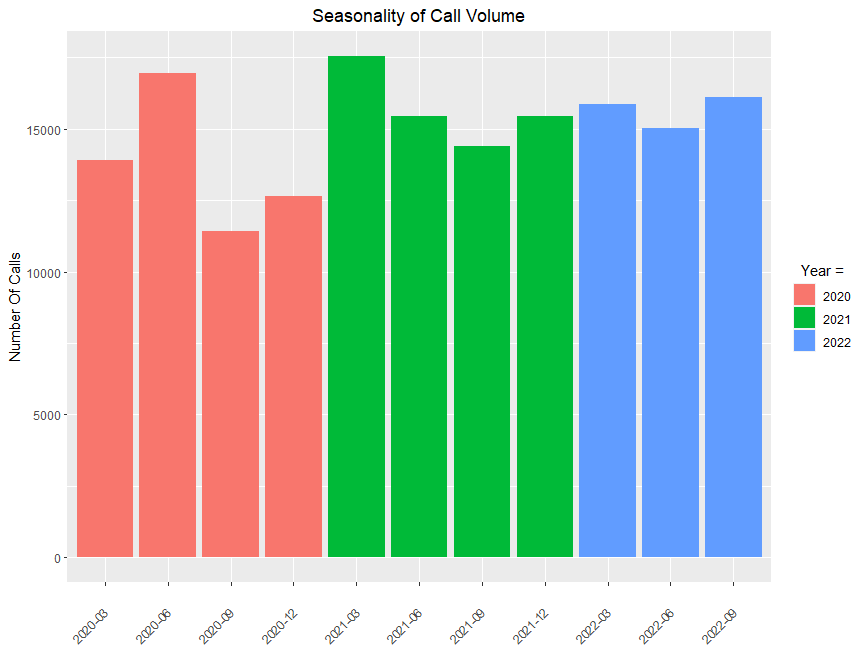
\includegraphics[width=\textwidth]{SeasonalityOfCallVolume.png}
  \caption{Seasonality Of Call Volume .}
  \label{fig:Seasonality}
\end{figure}
Here we do not see any clear pattern based on whether its winter, spring, summer, or fall. Overall, this was not too surpising.

I also created linear models to show the relationship between calls per agent and average waitime, holdtime, average goal met, and average 
interaction value. Average goal met was a variable created in relationship to the AnsweredGoalMet. AnsweredGoalMet was given in 1 and 0s, 
1 if the goal was hit and 0 if it was not hit. This variable is very fluid, as each company has its own reasoning for what they want their
goal time to be. Average Interaction Value was based off a variable that was created based on the InteractionOutcome. "Handled "got assigned 
1 as it was a positive outcome and -1 for "Abandoned" and "Leave Number" as they were deemed negative. The others were considered neutral, for example
"Not Specified", was given a 0. 

  Linear Regression is based off five key assumptions,
  \begin{enumerate}
  \item There is a Linear relationship,
  \item Multivariate normality,
  \item No or Little multicollinearity,
  \item No auto-correlation,
  \item Homoscedasticity
\end{enumerate} Multicollinearity refers to the occurrence of high intercorrelations among two or more independent variables in a multiple regression model.
To prevent this, I soley focus on one variable at a time when making my models on agents. Homoscedasticity is an assumption there is equal or similar variances in different groups being compared.
Logistic and Linear Regression Assumptions: Violation Recognition and Control goes into detail about this stating, "it is necessary to make a note about sample size for this type of regression model. In Linear
regression the sample size rule of thumb is that the regression analysis requires at least 20 cases per
independent variable in the analysis"\citep{schreiber2018logistic} 
I also used Pearson's correlation which states the following assumptions,
\begin{enumerate}
  \item The Variables must be continous,
  \item The Variables are paired,
  \item There should be an independece of cases,
  \item Both Variables should follow a normal distribution,
  \item There should be a linear relationship,
  \item Homoscedasticity,
  \item There should be no outliers,
\end{enumerate}
The Pearsons coefficient is given below:
\begin{equation}
  \label{eq:Pearson}
r= \Sigma((x_i - \bar{x})(y_i-\bar{y}))/(\sqrt{\Sigma{(x_i-\bar{x})^2}\Sigma{(y_i-\bar{y})^2}}),
\end{equation}
From here I then did a Correlation Plot:
\begin{figure}[H]
  \centering
  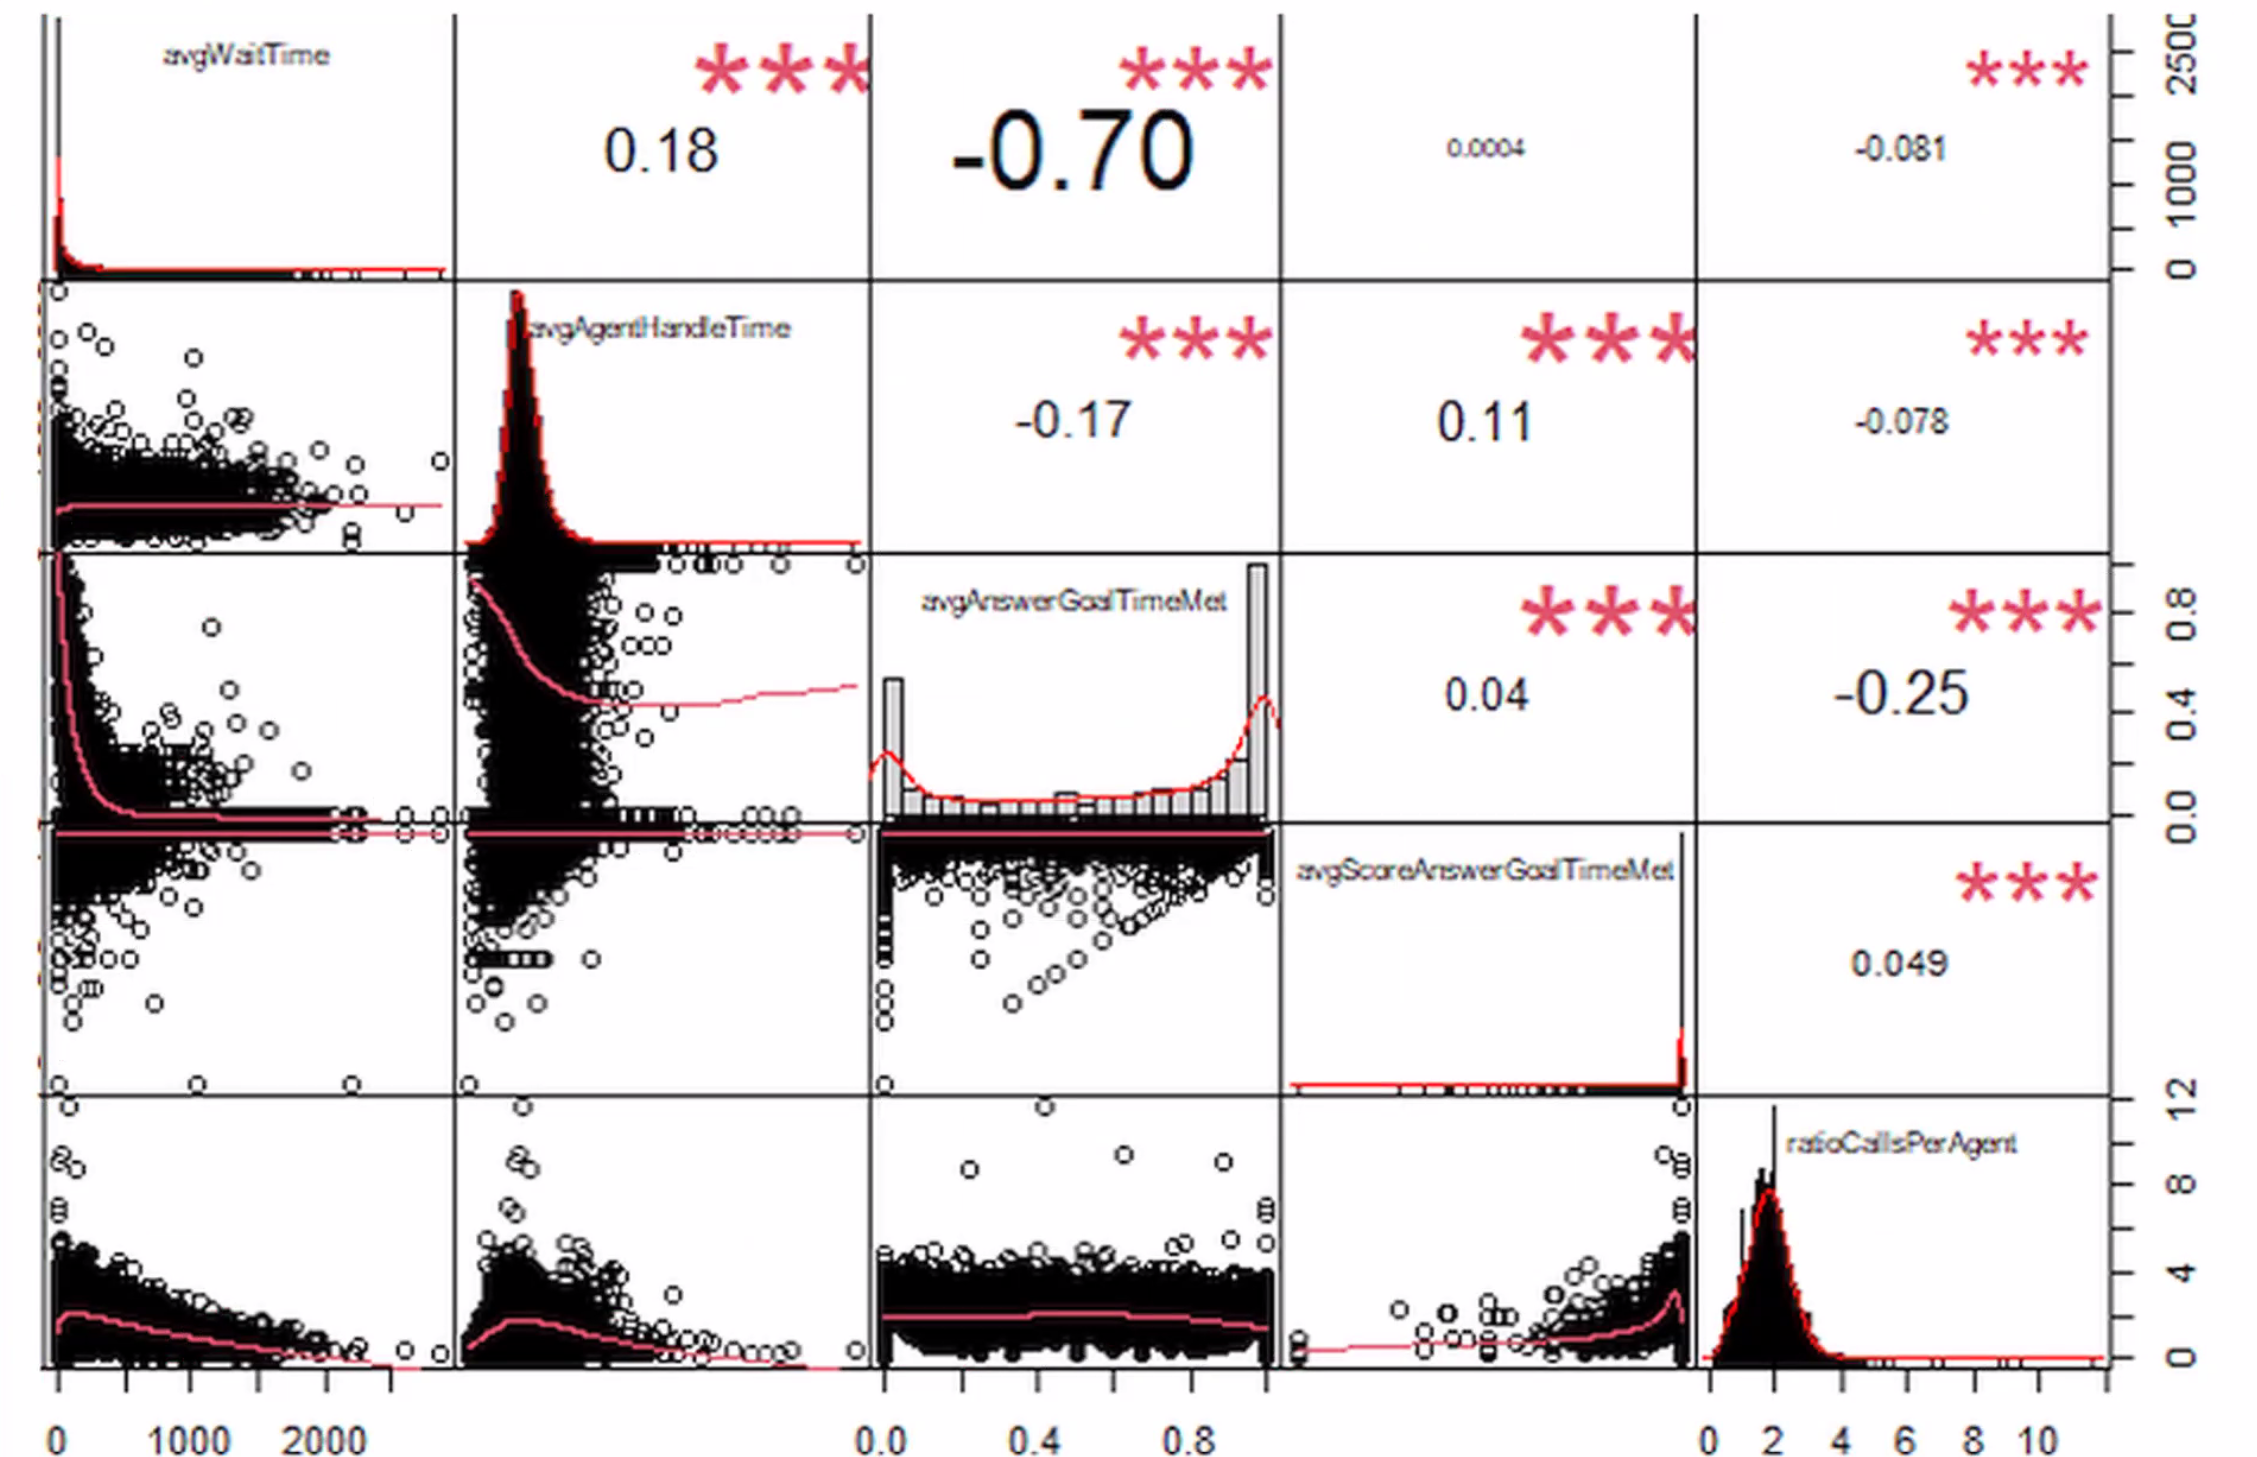
\includegraphics[width=\textwidth]{Correlation.png}
  \caption{Correlation Between Variables.}
  \label{fig:Correlation}
\end{figure}
Here we see that correlations between Average Wait Time, Average Handle Time, Average Answer Goal Time, Average Score Answer Goal Time Met, and Ratio Calls Per Agent.
We see that Calls Per Agent is correlated with all 4 variables in our models which was a great step to acheive. I then checked to see what the distribution was between calls per agent was throughout each day. 
  \begin{table}[H]
    \resizebox{\textwidth}{!} {
    \begin{tabular}{ l | l | l | l | l |}
      {\bf DayofWeek} & {\bf AvgNumCalls} & {\bf AvgNumAgents} & {\bf CallsPerAgent} & {\bf Num15Periods} \\
    \hline
    2 & 3.17 & 10.3 & 0.308 & 38 \\
    \hline
    3 & 3.25 & 9.81 & 0.331 & 39 \\
    \hline
    4 & 3.17 & 10.4 & 0.305 & 38 \\
    \hline
    5 & 3.08 & 10.1 & 0.306 & 37 \\
    \hline
    6 & 3.83 & 8.82 & 0.435 & 46 \\
    \hline
    7 & 1.25 & 6.33  & 0.197 & 15 \\
    \end{tabular}
    }
    \end{table}
Here we see that the Calls Per Agent is highest on Friday. This further proves that Friday is the busiest. Note that these are on 15 minute intervals,
so for example, the call center gets 3.17 calls every 15 minutes on average on a Monday. It was surpising to see that Friday was the second
lowest staffed day of the week. A possible suggestion to the company would be add an agent on Friday. Members may be calling about last minute
questions on Friday to enjoy the weekend and not have to call Saturday. In regards to Saturday, it is clear that is the least busiest day of the week,
this is not too suprising as many people like to sleep in on the weekends and not worry about financial issues. Monday through Thursday is relatively
consistant in all aspects. Note that the reason why the "num15minPeriods" variable is not the same is due to the outliers in the dataset where individuals
called either slightly before or after call center hours.
\section*{Simulation}
After seeing how consistent the call volume was and how big of a sample size I had, I decided to create a table and go off total calls and use averages to project call volume per weekday with the 
created variable called RatioDayPerWeek. This variable is the ratio of how many hours the call center was open historically on the day(Monday,Tuesday,Wednesday...) compared to all the total hours of all days.
I was able to produce this table:
\begin{table}[H]
  \resizebox{\textwidth}{!} {
  \begin{tabular}{ l | l | l | l | l |}
    {\bf DayofWeek} & {\bf numberofCalls} & {\bf AvgCallsPerDay} & {\bf RatioDayPerWeek} & {\bf ProjectedCallsPerDay} \\
  \hline
  2 & 79785 & 670 & 0.193 & 642 \\
  \hline
  3 & 89121 & 655 & 0.188 & 628 \\
  \hline
  4 & 89428 & 653 & 0.188 & 625 \\
  \hline
  5 & 84918 & 624 & 0.180 & 598 \\
  \hline
  6 & 95588 & 693 & 0.199 & 664 \\
  \hline
  7 & 24285 & 183 & 0.0525 & 175\\
  \end{tabular}
  }
  \end{table}
This table shows that Friday accounts for 19.9 percent of all the hours in the week the call center is open, while Saturday only accounts
5.25 percent of the hours. The only difference there is a different in ratio for Monday thru Thursday must be holidays, e.g. Thanksgiving. 
The Projected Calls Per Day simply came from the total calls per week * the RatioDayPerWeek. We can also see this approach worked relatively well in the forecasting model. 
We also see that the MAPE(Mean Absolute Percent Error) is 4.21 percent. For context, a MAPE score less than 5 is very accurate.

  Using this information, I was able to create a figure that showed the amount of expected calls per day per 15 minute intervals. 
  \begin{figure}[H]
    \centering
    \includegraphics[width=\textwidth]{Forecast15MinPeriods.png}
    \caption{This is the Forecast Per Day On a 15 Minute Intervals.}
    \label{fig:Forecast}
  \end{figure}
Here we see that distinct pattern similar to the historical graph. The graph peaks at 9am and then slowly trails throughout the day.
Note that the different colors represent the different days.

In regards to forecasting the number of agents, I created one last table to see if there is a difference in AgentHandleTime and WaitTime
by each 15 minute interval.
\begin{table}[H]
  \resizebox{\textwidth}{!} {
  \begin{tabular}{ l | l | l | l | l | l | l |}
    {\bf DayofWeek} & {\bf AvgNumCalls} & {\bf AvgNumAgents} & {\bf CallsPerAgent} & {\bf AvgAgentHandleTime} & {\bf AvgWaittime} & {\bf AvgInteractionValue}\\
  \hline
  2 & 2418 & 10.6 & 227 & 303 & 175 & 0.987 \\
  \hline
  3 & 2701 & 10.4 & 260 & 297 & 126 & 0.998\\
  \hline
  4 & 2710 & 10.7 & 254 & 297 & 80.9 & 0.987 \\
  \hline
  5 & 2573 & 10.2 & 253 & 289 & 87.1 & 0.988 \\
  \hline
  6 & 2897 & 9.93 & 292 & 293 & 88.2 & 0.987 \\
  \hline
  7 & 736 & 6.34 & 116 & 260 & 57.4 & 0.989\\
  \end{tabular}
  }
  \end{table}
  Overall, we see that Friday continues to be the busiest days in terms of call volume but the least staffed days. However, a glaring note
is how high the average waittime on Monday is. This may be suggesting that the subject matter of calls on Monday are more intense and urgent
then the subject matter on a day like Saturday. With such a high wait time but not a bigger handle time, this also may be suggesting that
employees are getting stressed out at lot more and may need more time to get themselves mentality ready to take the next call. It might be a good idea to add another employee for Mondays. 
The other days appear to be relatively normal and Saturday is functioning very efficiently. With a waittime less than 60 seconds, there is no reason to change the staffing model for
Saturday. 

  From there I ran Correlation between CallsPerAgent and the dependent variables. The Pearson Product Moment Correlation test can take a range of values from 1 to -1. A value of 0 shows there is no association between two variables. 
A value greater than 0 indicates a positive association, meaning as the value of the dependent variable increases so does the independent variable. A value less than 0 indicates a negative association, meaning as the dependent 
variable decreases so does the independent variable. The stronger the correlation between the variables the higher it is to 1 or -1.  The 4 dependent variables were Average Wait Time, Average Call Time, Average Goal Being Met, Average Interaction Value. 
The one dependent variable is CallsPerAgent. In this case, the Calltime is the same as Handletime, which is the combination of Wait time, Hold time, and Wrap Up Time. 
The Average Goal Being Met would be whatever the business establishes in seconds of  how long they would want a call center call to last. Average Interaction Value would be at what percentage 
they want calls being "Handled" or taken by an agent in anyway. 
\begin{table}[H]
  \resizebox{\textwidth}{!} {
  \begin{tabular}{ l | l |}
    {\bf Dependent Variable} & {\bf Correlation Coefficient}\\
  \hline
  Wait Time& 0.405 \\
  \hline
  Call Time& 0.238\\
  \hline
  Goal Met& -0.496  \\
  \hline
  Interaction Value& 0.484\\
  \end{tabular}
  }
  \end{table}
Typically, a Pearson's coefficient ranging between plus or minus .3 represents a small association, while a Pearson's coefficient
ranging between plus or minus .3 to .5 represents a medium association, and anything over plus or minus .5 represents a large association.
Wait Time and Calls Per Agent have a medium positive relationship which states as Calls Per Agent increases, so does the Wait Time for 
each Caller. Call Time and Calls Per Agent have a small positive relationship which states as Calls Per Agent increases, so does the 
Call Time. Goal Time and Calls Per Agents have the strongest relationship, in this case a negative medium relationship, which states as
Calls Per Agents increases, the Goal Being Met decreases. This means the Average Goal Time is nothing being hit consistently when Calls 
are increasing. Interaction Value and Calls Per Agent have a medium positive relationship. However, in theory, as calls increase there should
be more abandoned calls, but according to Pearsons Coefficient this is not the case. So while this relationship may not be a linear one,
I will still present a model for it.
  
  Here are the linear models:
  \begin{equation}
    \label{eq:Wait Time}
  AvgWaittime= -5.292 + 61.148*CallsPerAgent,
  \end{equation}
  \begin{equation}
    \label{eq:Call Time}
  AvgCallTime = -256.252 + 20.115*CallsPerAgent,
  \end{equation}
  \begin{equation}
    \label{eq:Goal Met}
  AvgGoalMet= 0.986 - 0.216*CallsPerAgent,
  \end{equation}
  \begin{equation}
    \label{eq:InteractionValue}
  AvgInteractionValue= 0.97 + 0.00989*CallsPerAgent,
  \end{equation}

  \begin{table}[H]
    \resizebox{\textwidth}{!} {
    \begin{tabular}{ l | l |}
      {\bf Dependent Variable} & {\bf R-squared Value}\\
    \hline
    Wait Time& 0.1642 \\
    \hline
    Call Time& 0.0569\\
    \hline
    Goal Met& 0.2458\\
    \hline
    Interaction Value& 0.234\\
    \end{tabular}
    }
    \end{table}
R-squared values range from 0 to 1. A R-squared value of 1 means that all movements of a variable are completely explained by another variable. 
Overall, the higher the R-squared the better.
\section*{Discussion}
Overall, the best agent model would be the model with the highest R-squared value and Pearson Coefficient. In this case, this would be
AvgGoalMet= 0.986 - 0.216*CallsPerAgent. A close second place would be AvgWaittime= -5.292 + 61.148*CallsPerAgent, as it had a decent 
Pearson coefficient and R-squared value. Unfortunately, because of the Pearsons Coefficient I would not recommend the Interaction Value model however even though it had a good 
r-squared value. Overall the other 3 models are would suggest to an individual to use to determine how many agents
there business to have. Unfortunately, there are so many aspects to just this. In regards to a business perspective, the call center must have
a budget so it is a difficult road to navigate. But, I believe it is possible to find a balance in between to ultimately maximize efficiency.
We were also able to forecast call center volume using historical data and the ratio of how many hours the call center is open compared to each day to
a week. 

  The biggest limitation I would say was that there is no right answer to answering the calls per agent problem. In an ideal situation, you would have
plenty of agents so waittime is completely reduced. However that is not efficient or plausible. I also do wish I knew the answer to what
the actual Goal time was, this would help me be more confident in my model I created. I did try to create a model to the ratio of Calls Per Agent,
but Unfortunately the parameters estimates were simply just inaccurate. 

Another challenge was dealing with the time complexities in the dataset. There are 6 days of the week, 47 15-minute-intervals across any day, which each occur a different number of times,
and 213 15-minute-intervals across each week. This does not average out between days of the week. There was also 139 weeks in the data, 971 days in all the data, and
27377 15-minute-intervals in all the data. So this fails to account for discrepancies in between days of the week. Also, Call time and any values
about the all are data explicitly about the call so they are in the row in the itself, so we have to normalize the number of agents by number of calls During
that period recorded before we run a model comparing both values. So overall, there was a lot of data cleaning and preparing needed in this dataset, that
took time away from the data analysis.

  I still believe this study can be expanded on. Monday has a wait time of 175 seconds while Friday has a wait time of 88.2 seconds. Possibly multivariate regression technqiues could be used to model the number of agents needed.
With the data at my hands, I could also try to answer questions such as if call length is dependenton call reason or even do an analysis on if all agents are performing
on the same level. In detail, \citep{evensen1999effective} believes that "Since the primary interface between a financial institution and its customer is a service
representative, this element strongly influences an institution's ability to deliver quality service.An organization’s human resource (HR) practices effect how well its employees are able to perform. More
specifically, human resource practices directly influence how knowledgeable an employee is about the product offering, whether or not an employee is empowered to resolve customer issues in real time, and the
level of turnover within the organization". This is an interesting point as one could analyze how Human Resources Data plays a role in qualities like AgentHandleTime that reflects on the agents performance. Another interesting question to look into was the abandonment 
rate and if how many times someone will call back the same day. I personally did not look into the chat feature that much, but I am sure that there is some interesting information like if people tend to reuse often.
Another topic of interest is how does call center volume change on when there is an information technology problem such as the online banking services having an outage?

\bibliographystyle{chicago}
\bibliography{Citations.bib}
\end{document}